\chapter{Estrutura e funcionamento\label{cap:detalhamento-projeto}}

    \section{Processo de instalação\label{sec:processo-instalacao}}
        O \emph{Framework Lothus\{PHP\}} permite ao desenvolvedor a possibilidade de escolha entre dois níves de aplicação. O primeiro nível permite a instalação do \emph{Framework} da forma mais simples, instalando utilitário focados em um desenvolvimento direcionado ao backend do projeto, integrando facilidade a troca de informações com o banco de dados, desenvolvimento através do MVC, URLs amigáves e sistemas de templates.

        Essa instalação é feita através do repositório remoto \emph{Github}, que se encontra no seguinte endereço online:

        \emph{https://github.com/guilouro/Lothus-PHP}

        O Github permite duas formas de download de um projeto: fazendo o downloand de um arquivo comprimido em .zip diretamente do site ou utilizando um sistema de versionamento de arquivos para fazer o clone do mesmo. Neste projetos iremos usar o \emph{Git} como sistema de versionamento. Para fazer o clone utilizando o git executamos a seguinte linha de comando no terminal Unix ou cmd Windows:

        \textbf{\$ git clone https://github.com/guilouro/Lothus-PHP.git}

        Ao executar essa linha de comando, uma nova pasta será criada com o nome de Lothus-PHP. Dentro desta nova pasta estará todo o projeto para iniciar o desenvolvimento utilizando o \emph{Framework Lothus\{PHP\}}. O próximo capítulo será responsável pela apresentação das pastas existentes dentro do projeto.



    \section{Estrutura de pastas e arquivos\label{sec:estrutura-pastas}}
        Neste capítulo será apresentado a estrutura de pastas do \emph{Framework Lothus\{PHP\}} juntamente com o processo de criação e funcionamento de cada etapa.

        Ao clonar o projeto utilizando o git, como visto no capítulo anterior, será gerada uma estrutura de pastas dentro da pasta Lothus-PHP.

        \begin{figure}[!htb]
            \centering
            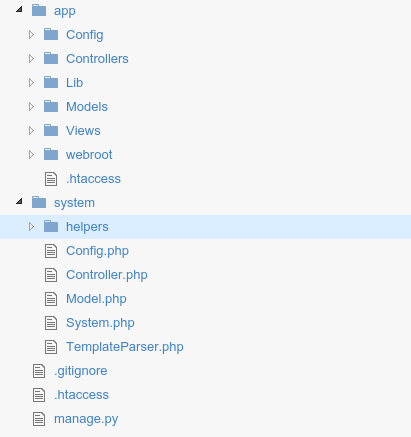
\includegraphics[scale=0.8]{pastas.jpg}
            \caption{\small Estrutura do projeto}
            \label{cap:sass}
        \end{figure}

        Neste primeiro momento já ocorre uma pequena divisão do projeto onde a pasta \emph{app} é responsável por gerenciar a aplicação e a pasta \emph{system} responsável pelo \emph{core}, ou seja, gerenciamento interno do framework. Em sua raiz existe, além dessas duas pastas, três importantes arquivos para o projeto, que são:

        \begin{itemize}
            \item \textbf{.gitignore}: Um arquivo que faz parte da configuração do git e é responsável por guardar, linha por linha, todos os arquivos ou pastas serão ignorados pelo git no momento de fazer o versionamento do projeto. Isso evita o acumulo de arquivos desnecessários, que são gerados automaticamente, no pacote de instalação do Framework.

            \item \textbf{.htaccess}: Arquivo que é lido antes do index.php e tem a responsabilidade de criar a rota inicial do projeto, fazendo o direcionamento para o arquivo correto na inicialização do sistema.

            \begin{figure}[!htb]
                \centering
                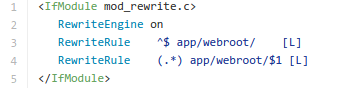
\includegraphics[scale=0.8]{htaccess1.jpg}
                \caption{\small Estrutura do htaccess na raiz do projeto}
                \label{cap:sass}
            \end{figure}

            \item \textbf{manage.py}: Trata-se de um script de linha de comando capaz de gerar novos arquivos baseados na arquitetura de funcionamento do \emph{Framework}. A imagem abaixo ilustra o uso básico da ferramenta.

            \begin{figure}[!htb]
                \centering
                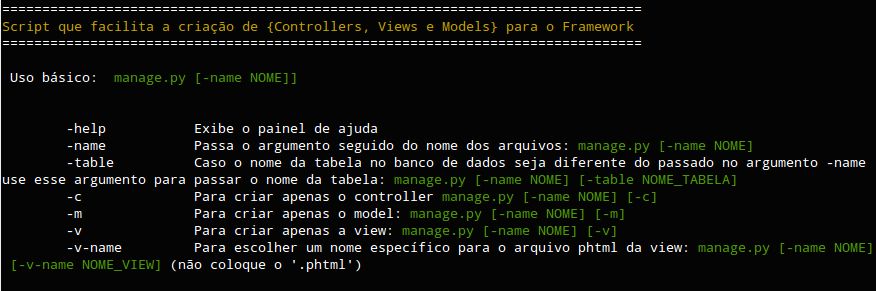
\includegraphics[scale=0.5]{manage.jpg}
                \caption{\small Regras para uso básico do manage.py}
                \label{cap:sass}
            \end{figure}


        \end{itemize}

    \section{Sistema\label{sec:system-core}}

        O Framework recebe um primeiro nível de divisão no processo de criação do mesmo, que é a divisão do Sistema par a Aplicação o sistema fica todo centralizado na pasta \emph{system}, e é onde contém o motor do \emph{Framework}, nele estão todas as classes responsáveis pelas regras de funcionamento do projeto, tanto nas requisições HTTP, passando por padronização de Controllers, Views até chegar ao relacionamento com o banco de dados. Todas essas funcionalidades estão divididas entre classes e arquivos que serão detalhados ao longo deste capítulo.

    \begin{figure}[!htb]
        \centering
        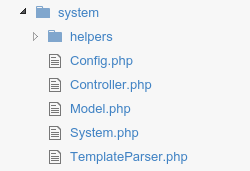
\includegraphics[scale=0.6]{system-path.jpg}
        \caption{\small Estrutura interna da pasta system}
        \label{cap:sass}
    \end{figure}



        \subsection{Config\label{sub:system-config}}

            A Classe \emph{Config} é responsável pela configuração inicial de qualquer projeto que faz uso do \emph{Lothus\{PHP\}}. Ela tem a responsabilidade de definir qual \emph{View} será iniciada ao acessar o link do sistema e também se responsabiliza em definir se será exibido ou não um \emph{debug} para o desenvolvedor.

            \emph{}

            O arquivo \emph{Config.php} possui a seguinte estrutura:

            \emph{}

\begin{lstlisting}
class Config {
    public  $_Index = "home";
    private $error = TRUE;

    protected function ERROR($pag){}
}
\end{lstlisting}


        \begin{itemize}
            \item\textbf{\$\_Index}: É uma variável \textbf{pública} que recebe, como string, o nome do \emph{Controller} padrão a ser requisitado pelo sistema no caso de a URL não ter, explicitamente, este valor.

            \item\textbf{\$error}: Trata-se de uma \textbf{privada} váriavel booleana, que funciona como uma chave para exibir um erro para o desenvolvedor ou direcionar o usuário para uma página 404, no momento em que for acessada alguma página inexistente. No caso de \textbf{\$error = TRUE} será exibido uma mensagem de alerta ao desenvolvedor sobre alguma falha nos padrões do \emph{Framework}. Caso \textbf{\$error = FALSE} o usuário será redirecionado para uma página de \emph{erro 404}

            \item\textbf{ERROR(\$pag)}: É um método protegido, que recebe como parâmetro o nome da página que não foi encontrada no sistema. Sua funcionalidade é, inicialmente, verificar se a variável \textbf{\$error} é \textbf{TRUE} \emph{(Verdadeiro)} ou \textbf{FALSE} \emph{(False)}, para posteriormente, direcionar o usuário para a página de erro padrão do sistema ou exibir uma mensagem dizendo se o erro foi causado pela falta de um \emph{Controller} ou de uma \emph{Action} para o sistema.
        \end{itemize}

        \emph{}

        \emph{}

        A lógica de programação aplicada a este método é a seguinte:

        \emph{}

\begin{lstlisting}
protected function ERROR($pag) {
    if($this->error) {
        /* Erro em Controller ou Action */
    } else {
        /* Redirecionamento */
    }
}
\end{lstlisting}


        \subsection{System\label{sub:system-sis}}

            O projeto é iniciado com a primeira chamada sendo referenciada à classe \emph{System} que tem como herança os métodos e atributos, que não são privados, da classe \emph{Config}. Sua principal funcionalidade é interpretar o padrão de URL criado para o Framework e fazer a separação para a camada correta de Controllers e actions com seus respectivos parâmetros, quando houver.

            O \emph{Lothus\{PHP\}} usa um padrão de url denominado \textbf{url amigável}, que facilita tanto a leitura dos mecanismos de buscas quanto a leitura do próprio usuário, além de padronizar todos os projetos desenvolvidos pelo \emph{Framework}.

            A URL segue o seguinte padrão:

            \emph{http://urldosite.com.br/\{Controller\}/\{Action\}/\{n-parametros\}}

            \begin{itemize}
                \item\textbf{Controller:} Classe controller referente à página acessada
                \item\textbf{Action:} Método existente nessa mesma classe
                \item\textbf{n-parametros:} Será passado como argumento para a o método desta mesma classe controller.
            \end{itemize}

            Todos esses itens serão abordados corretamento no momento em que for descrito o funcionamento das classes de Aplicação do projeto.

            Pode se explicar que a classe system, ao ser invocada, recebe a URL via GET e através de alguns métodos essa URL é desmembrada, as variáveis da classe são definidas e por fim o projeto é inicia, como demostrada na estrutura da classe logo abaixo.

\begin{lstlisting}
class System extends Config {

    public $_url;
    private $_explode;
    public  $_controller;
    public  $_action;
    public  $_params;

    public function init(){}
    private function setUrl(){}
    private function setExplode(){}
    private function setSlug($w){}
    private function setController(){}
    private function setAction(){}
    public function setParams(){}
    public function setGets(){}
    public function run(){}
}
\end{lstlisting}

            A classe possui alguns atributos responsáveis por guardar determinadas informações a serem utilizadas em diversas etapas de sua leitura. Esses atributos tem suas responsabilidades descritas abaixo.

            \begin{itemize}
                \item\textbf{\$\_url}: Atributo público que receberá a url atual como string.
                \item\textbf{\$\_explode}: É um vetor privado que receberá, em cada uma de sua posição, uma parte da URL que se utiliza da \emph{"/"} como regra de separação.
                \item\textbf{\$\_controller}: Atributo público que guardará o nome do Controller a ser usado.
                \item\textbf{\$\_action}: Atributo público que guardará o nome da Action a ser usada.
                \item\textbf{\$\_params}: Vetor público que guardará todos os parâmetros passados pela URL.
            \end{itemize}

            Esses valores são atribuídos através dos métodos que além de atribuir fazem uso dessas mesmas variáves da classe, como descrito nos elementos de cada método abaixo.
.
            \begin{itemize}

                \item\textbf{init()}: Primeiro método a ser chamado, explicitamente, pela classe e responsável por fazer a chamada de todos os métodos que fazem as atribuíções a todas as variáves dessa classe.
\begin{lstlisting}
public function init() {
    $this->setUrl();
    $this->setExplode();
    $this->setController();
    $this->setAction();
    $this->setParams();
    $this->setGets();
}
\end{lstlisting}

                \item\textbf{setUrl()}: Responsável por atribuir a string da URL atual para a variável \textbf{\$\_url}. Caso a URL passada não tenha, explicitamente um controller e uma action, será atribuído o valor da variável \textbf{\$\_Index}, que é uma herança da classe Config, juntamente com a action padrão \textbf{index\_action}.
\begin{lstlisting}
private function setUrl() {
    $this->_url = (isset($_GET['url']) ? $_GET['url']  :
        $this->_Index . "/index_action" );
}
\end{lstlisting}

                \item\textbf{setExplode()}: Método que atribui ao array\emph{(Vetor)} \textbf{\$\_explode} os valores passados para a variável \textbf{\$\_url} e delimitados pela barra\emph("/").

\begin{lstlisting}
private function setExplode(){
    $this->_explode = explode("/", $this->_url);
}
\end{lstlisting}

                \item\textbf{setController()}: Define qual controller será usadado para a requisição atual, através do primeiro índice do vetor \textbf{\$\_explode}

\begin{lstlisting}
private function setController(){
    $this->_controller = $this -> setSlug($this -> _explode[0]);
}
\end{lstlisting}

                \item\textbf{setAction()}: Define qual action será usadado para a requisição atual, através do segundo índice do vetor \textbf{\$\_explode}. Caso não exista, será atribuído o valor \textbf{"index\_action"}.

\begin{lstlisting}
private function setAction(){
    $this->_action = $this -> setSlug(
        !isset($this->_explode[1]) ||
        $this->_explode[1] == null ||
        $this->_explode[1] == 'index' ? 'index_action' :
        $this->_explode[1]);
}
\end{lstlisting}

                \item\textbf{setParams()}: Responsável por criar o vetor para todos os parâmetros passados pela URL atual. Parâmetros esses que são definidos por todos o valores passados além do controller e action na string da URL.

\begin{lstlisting}
public function setParams(){
    unset($this->_explode[0], $this->_explode[1]);
    if( end( $this->_explode ) == null )
        array_pop($this->_explode);
    $this->_params = $this->_explode;
}
\end{lstlisting}

                \item\textbf{setGets()}: Verifica a aparição da requisição GET no HTTP da página atual e define o vetor \textbf{\$\_GET} do PHP com seus respectivos valores.

\begin{lstlisting}
public function setGets(){
    $url = $_SERVER['REQUEST_URI'];
    $url = explode("?", $url);
    if(isset($url[1])) {
        $urlParams = explode("&", $url[1]);
        foreach ($urlParams as $g) {
            $get = explode("=", $g);
            $_GET[$get[0]] = $get[1];
        }
    }
}
\end{lstlisting}

                \item\textbf{setSlug(\$w)}: É responsável por verificar se o item \textbf{\$w} possui duas ou mais palavras separadas por ífem. Caso exista, esse método retira os ífens e transforma todas essas palavras em apenas uma no modo \emph{CamelCase}.

\begin{lstlisting}
private function setSlug($w){
    $arr = explode("-", $w);
    for ($i=1; $i < count($arr); $i++) {
        $arr[$i] = ucfirst($arr[$i]);
    }
    $slug = implode("", $arr);
    return $slug;
}
\end{lstlisting}

                \item\textbf{run()}: É o método responsável por carregar o controller e a action com todos os parâmetros, caso eles existam. Se algum desses objetos não forem encontrado, o método \textbf{\$ERROR}, herdado da classe \emph{Config}, é chamado para exibir a mensagem adequada ao usuário.

            \end{itemize}



        \subsection{Helpers\label{sub:system-helper}}
            São classes que auxiliam o desenvolvedor no andamento do projeto, podendo ou não ser utilizadas em determinadas aplicações. O \emph{Framework} vem com algumas classes em sua instalação, podendo ser adicionadas outras se o desenvolvedor sentir necessidade. As classes se encontram dentro da pasta \textbf{helpers} e segue um padrão de nomenclatura que é o nome da classe acompanhada da palavra \emph{Helper}. Para uma classe chamada \textbf{Email} teria que ter a seguinte nomenclatura: \textbf{EmailHelper}.

            O projeto acompanha algumas classes que serão descritas logo abaixo:

            \begin{itemize}
                \item\textbf{AuthHelper}: Auxilia na autenticação de usuários para projetos que possuem áreas restritas. Ela se responsabiliza em fazer o login do usuário no sistema de forma segura, comparando a senha digitada com a que possui no banco de dados através da criptografia \textbf{sha512} e iniciando uma sessão para o usuário. Possui um métdo de logout, onde finaliza uma sessão com o usuário e o desconecta da área restrita do sistema. Além de possuir métodos que ajudam no controle de páginas protegidas, fazendo a verificação da permissão cada vez que o usuário tenta acessar a mesma.

                \item\textbf{EmailHelper}: Classe auxiliadora para envio de emails. Extende à classe \emph{PHPMailer} e trabalha como uma facilidadora para esta, que é uma ferramenta avançada para envio de emails em \emph{php}.

                \item\textbf{ImageHelper}: Esta é uma classe para otimização e salvamento de imagens nos projetos. Ela pode trabalhar tanto com imagens enviadas por um formulário quanto imagens provenientes de algum link da internet. Sua estrutura é formada apenas por um construtor e mais 3 métodos públicos. Ós métodos \textbf{ResizeByUrl} e \textbf{ResizeByUpload} salvam o arquivo de imagem na pasta especificada através do construtor da classe e retornam o nome gerado para o arquivo pelo método \textbf{Rename}. Esse nome é gerado para evitar a criação de imagens caractéres especiais em seu nome evitando inclusive, sobrescrever imagens com o mesmo nome. A classe obedece a seguinte estrutura descrita abaixo:

\begin{lstlisting}
class ImageHelper {

    private $_ALTURA_PADRAO;
    private $_pasta;

    /*
     * Metodo construtor
     * @param $pasta = Nome da pasta para upload
     * @param $altura_padrao = Definir uma altura padrão para os arquivos
     */
    function __construct($pasta, $altura_padrao = null) { }

    /*
     * Metodo ResizeByUrl
     * Salva uma imagem a partir de um link
     * @param $url = Url da imagem a ser salva
     * @param $altura = Definir uma altura para a imagem atual, caso seja diferente da altura padrão
     */
    public function ResizeByUrl($url, $altura = null) { }

    /*
     * Metodo ResizeByUrl
     * Salva uma imagem a partir de upload
     * @param $imagem = ex: $_FILES['imagem']
     * @param $altura = Definir uma altura para a imagem atual, caso seja diferente da altura padrão
     */
    public function ResizeByUpload($imagem, $altura = null) { }

    /*
     * Metodo Rename
     * Remove acentos, espaços e caracteres especiais e cria um nome aleatório.
     * @param $string = string a ser limpa
     */
    public function Rename( $string ) { }
}
\end{lstlisting}

            \item\textbf{PaginationHelper}: Classe capaz de dividir um conteúdo vindo do banco de dados em diversas páginas através de uma paginação. A classe permite, ao ser instanciada, receber o nome da tabela no banco de dados que será feita a consulta. Essa consulta possibilita ao desenvolvedor escolher quantos itens serão exibidos por páginas e a ordem de exibiçao. Além dessa exibição ela fornece alguns métodos auxiliares onde se pode ter o retorno da página ou url atual. A classe possui uma estrutura bem simples como mostrada abaixo.

\begin{lstlisting}
class PaginationHelper
{
    private $_model;
    private $_limite;
    private $_paginaAtual;
    private $_inicio;
    private $_total_registros;

    /**
     * Classe para paginação
     * @param String $tabela tabela no banco de dados para a consulta
     */
    function __construct( $tabela ) { }

    /**
     * Pega a quantidade total de páginas de acordo com a lista
     * @return int retorna a quantidade de páginas
     */
    public function totalPaginas() { }

    /**
     * Responsável por fazer a consulta limitada
     * para a paginação e definição de alguns atributos
     * @param  Array $arr parâmetros SQL. 'where' , 'orderby'
     * @return Array      retorna a consulta limitada
     */
    public function consulta(Array $arr = null) { }

    /**
     * Retorna a página atual captura
     * @return int
     */
    public function getPaginaAtual() { }

    /**
     * Gera url atual
     * @return string retorna a url até a parte da pagina
     */
    public function getUrl() { }

    /**
     * Cria a view para exibição da paginação
     * @param  string $classe define a classe da div que engloba a paginação
     * @return string
     */
    public function view($classe = "pagination pagination-centered") { }
}
\end{lstlisting}

            Ao fazer a chamado do método \textbf{view()} no template do sistema, um componente de paginação é criado de acordo com a quantidade de páginas existente na sessão atual. Esse método, por padrão, cria o componente com uma classe de \emph{css} referente ao framework \emph{Bootstrap}. Com isso o componente passa a ter uma formatação adequada para uma paginação.

            \begin{figure}[!htb]
                \centering
                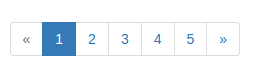
\includegraphics[scale=1]{paginacao.png}
                \caption{\small Componente de paginação criado por PaginatioHelper}
                \label{cap:paginaca}
            \end{figure}


            \item\textbf{RedirectHelper}: Simples classe que fornece a possibilidade de trabalhar com redirecionamento dentro do projeto. Possui métodos para retorno de url, \emph{Controller} atual e \emph{Action} atual. Seu métodos principais são os de redirecionamento, tomando como base o \emph{controller}, a \emph{action} ou ambos como ponto de destino para este redirecionamento. A classe e seus principais métodos podem ser vistas no modelo abaixo:


\begin{lstlisting}
class RedirectHelper {
    ...

    /**
     * Retorna o controller atual
     * @return (String)
     */
    public function getCurrentController() { }

    /**
     * Retorna a action atual
     * @return (String)
     */
    public function getCurrentAction() { }

    /**
     * Redireciona para o controller especificado
     * @param  (String) nome do controller
     * @return void
     */
    public function goToController( $controller ) { }

    /**
     * Redireciona para a action especificada
     * @param  (String) nome da string
     * @param  (boolean) para usar parâmetro global
     * @return void
     */
    public function goToAction( $action, $paramsGlobal = FALSE ) { }

    /**
     * Redireciona para controller e action especificada
     * @param  (String) nome controller
     * @param  (String) nome action
     * @return void
     */
    public function goToControllerAction( $controller, $action ) { }

    ...

}
\end{lstlisting}

            \end{itemize}



        \subsection{Controller\label{sub:system-controller}}
            Essa classe recebe a \emph{System} como herança e possui, inicialmente, dois métodos e um atributo. Sua função é guardar o template que será usado e compitar a view para o sistema. A estrutura da classa está descrita abaixo.


\begin{lstlisting}
class Controller extends System {

    public $_layout = 'default';

    protected function view($nome_pagina, $vars = null) { }

    public function init() { }
}
\end{lstlisting}

            \begin{itemize}
                \item\textbf{\$\_layout}: Atributo público para definir o template base da página a ser carregada.
                \item\textbf{view(\$nome\_pagina, \$vars \= null)}: Método responsável por atribuir o template da view ao template base, e recebe como primeiro parâmetro \emph{(\$nome\_pagina)} o nome do arquivo do template a ser utilizado. O Método possui um segundo parâmetro \emph{(\$vars)} opcional, que é capaz de receber um vetor e distribuí-lo em variáveis para ser utilizada no template carregado.

                \item\textbf{init()}: É o primeiro método a ser chamado no momento da criação do Controller. Ele pode ser ou não implementado dentro de cada controller criado e é o primeiro método a ser executado sempre que carrega uma página.
            \end{itemize}


        % \subsection{Url amigável e o padrão MVC\label{sub:url-amigavel}}

        \subsection{Model\label{sub:system-model}}
            Classe responsável por fazer a comunicação entre aplicação e banco de dados. Utizando, como padrão, o módulo nativo do php chamado \emph{PDO}. Esta classe segue a seguinte estrutura descrita abaixo.


\begin{lstlisting}
class Model {
    protected $db;
    public    $_tabela;
    public    $_fk;

    public function __construct()  { }

    public function insert( Array $dados, $debug = FALSE ) { }

    public function read( $where = null , $limit = null ,
        $offset = null , $orderby = null, $debug = FALSE ) { }

    public function readLine( $where = null , $limit = null ,
        $offset = null , $orderby = null, $debug = FALSE ) { }

    public function update( Array $dados, $where, $debug = FALSE ) { }

    public function delete( $where ) { }

    public function consulta($sql, $debug = FALSE) { }

    public function consultaLinha ( $sql , $debug = FALSE ) { }

    public function consultaValor ( $sql , $debug = FALSE ) { }

    public function populateFK() { }

}
\end{lstlisting}

            \begin{itemize}
                \item\textbf{\$db}: Atributo protegido que se torna uma instância da classe \emph{PDO}, capaz de fazer o processo de envio e recebimento de dados entre aplicação e banco de dados. Este objeto é instanciado através do construtor da classe.

                \item\textbf{\$\_tabela}: Atributo público que guarda uma \emph{string} como o nome da tabela, existente no banco de dados, que será manipulada pela classe.

                \item\textbf{\$\_fk}: Atributo que recebe um vetor, no caso de existeir relações entre tabelas, ligadas com chave estrangeira.

                \item\textbf{insert(Array \$dados, \$debug\=FALSE)}: Método público, responsável por fazer a inserção de novos dados na tabela que está especificada na classe. O metodo \emph{insert} recebe como parâmetro um vetor, denominado \textbf{\$dados}, com os dados a serem inseridos. Este vetor, por padrão precisa conter no mínimo uma chave e um valor, onde a chave será o nome da coluna e o valor será o conteúdo desta coluna a ser inserido no banco de dados. O retorno deste método é o \emph{Id} da linha inserida caso a ação seja bem sucedida, do contrário retornará um valor nulo. O método permite um segundo parâmetro, opcional, chamado textbf{\$debug}. Debug aceita valores \emph{booleanos} onde, se receber \textbf{true} ele imprime na tela a string completa que faz a interação naquele momento com o banco de dados, no caso de \textbf{false} ele não faz nada. Por padrão \textbf{\$debud} é iniciado como falso.

                \item\textbf{read(\$where\=null, \$limit\=null, \$offset\=null, \$orderby\=null, \$debug\=FALSE)}: Método público, responsável pela consulta direcionada à tabela especificada na classe. Este método fornece ao desenvolvedor a possibilidade de passar alguns parâmetros, responsáveis pela filtradem dos dados retornados. A passagem de parâmetro é opcional e possui nomenclaturas intuitivas que auxiliam no entendimento das funcionalidades. Por padrão o método \emph{read()}, sem passar parâmetro algum, retorna um vetor com dados relacionado a uma consulta completa e sem filtros da tabela especificada. O restorno pode ser filtrado definindo os parâmentros do método.
                \begin{itemize}
                    \item\textbf{\$where}: Condição a ser tratada pela clausula \emph{WHERE} do mysql na consulta solicitada.
                    \item\textbf{\$limit}: Responsável por determinar o ponto final, através da quantidade de linhas retornadas.
                    \item\textbf{\$offset}: Responsável por determinar o ponto inicial, através da quantidade de linhas retornadas.
                    \item\textbf{\$orderby}: Nome da coluna em que a consulta usa como base para ordenação do resultado.
                    \item\textbf{\$debug}: Imprime na tela a string completa que faz a interação naquele momento com o banco de dados.
                \end{itemize}

                \item\textbf{readLine(\$where\=null, \$limit\=null, \$offset\=null , \$orderby\=null, \$debug\=FALSE)}: Tem a mesma caracterísca do método \emph{read()}, porém o seu retorno é de um vetor com apenas um indice baseado em uma consulta de uma linha do banco de dados.

                \item\textbf{update(Array \$dados, \$where, \$debug\=FALSE)}: Atualiza os dados em determinada linha de uma tabela, utilizado o \emph{UPDATE} do mysql. O método possui a necessidade de passagem de dois parâmetros obrigatórios e da a opção de um terceiro parâmetro não obrigatório, são eles:
                \end{itemize}
                    \item\textbf{\$dados}: Parâmetro obrigatório que possui um vetor com os dados a serem atualizados no banco de dados.
                    \item\textbf{\$where}: Parâmetro obrigatório com a condição a ser utilizada pelo \emph{WHERE} do mysql, com a responsabilidade de tratar em quais linhas da tabela serão feitas as subistituições solicitadas.
                    \item\textbf{\$debug}: Imprime na tela a string completa que faz a interação naquele momento com o banco de dados.
                \begin{itemize}

                \item\textbf{delete(\$where)}: Exclui uma linha do banco de dados referente à condição passada pelo parâmentro \textbf{\$where}

                \item\textbf{consulta(\$sql, \$debug\=FALSE)}: Este método permite ao desenvolvedor passar uma string completa de sql para retornar um conjunto de linhas específicos a essa consulta. O método recebe as regras da consulta, faz a busca no banco de dados e retora um vetor com todas as linhas da tabela referente à consulta. Esse método não utiliza a variável \$\_tabela como referência ao banco de dados e aceita dois parâmetros, que são os seguintes:
                \end{itemize}
                    \item\textbf{\$sql}: Parâmetro obrigatório que recebe a string completa de consulta ao banco de dados.
                    \item\textbf{\$debug}: Imprime na tela a string completa que faz a interação naquele momento com o banco de dados.
                \begin{itemize}

                \item\textbf{consultaLinha(\$sql, \$debug\=FALSE)}: Este método permite ao desenvolvedor passar uma string completa de sql para retornar apenas uma linha referente a essa consulta. O método recebe as regras da consulta, faz a busca no banco de dados e retora um vetor uma linha da consulta efetuada. Esse método não utiliza a variável \$\_tabela como referência ao banco de dados e aceita dois parâmetros, que são os seguintes:
                \end{itemize}
                    \item\textbf{\$sql}: Parâmetro obrigatório que recebe a string completa de consulta ao banco de dados.
                    \item\textbf{\$debug}: Imprime na tela a string completa que faz a interação naquele momento com o banco de dados.
                \begin{itemize}

                \item\textbf{consultaValor(\$sql, \$debug\=FALSE)}: Este método permite ao desenvolvedor passar uma string completa de sql para retornar apenas um valor referente a essa consulta. O método recebe as regras da consulta, faz a busca no banco de dados e retora um único valor da consulta efetuada. Esse método não utiliza a variável \$\_tabela como referência ao banco de dados e aceita dois parâmetros, que são os seguintes:
                \end{itemize}
                    \item\textbf{\$sql}: Parâmetro obrigatório que recebe a string completa de consulta ao banco de dados.
                    \item\textbf{\$debug}: Imprime na tela a string completa que faz a interação naquele momento com o banco de dados.
                \begin{itemize}

                \item\textbf{populateFK()}: Caso a variável \textbf{\$\_fk} possua um vetor como valor, este método é capaz de percorrer cada valor, executar o método \emph{read()} referente a cada tabela e popular o retorno para uma variável como mesmo nome da tabela do banco de dados.

            \end{itemize}

        \subsection{Template\label{sub:system-template}}


    \section{Aplicação\label{sec:app}}

        falar do htaccess

        \subsection{Config\label{sec:app-config}}

        \subsection{Model\label{sec:app-model}}

        \subsection{View\label{sec:app-view}}

        \subsection{Controller\label{sec:app-controller}}

        \subsection{Lib\label{sec:app-lib}}

        \subsection{webroot\label{sec:app-lib}}


        \subsection{Controller\label{sec:app-controller}}


    \section{Divisão Backend - frontend\label{sec:back-front}}


        \subsection{Comandos do Grunt\label{sub:comandos-grunt}}
